\clearpage
\section{Cracking Pattern caused by Pure DEF Expansion}

\subsection{DEF Expansion Simulation of Single Aggregate Case}

In this section, similar as in ASR cases, simulation of DEF expansion on $10 \times 10 \times 10$ mm size model(Figure \ref{mmmm}) with only single aggregate in center of it is presented. As for the scale we considered here is relatively small, uniformed expansion is applied. 0.0003 initial strain is given to all paste interfaces uniformly in this simulation.

\begin{figure}[h!]
\centering

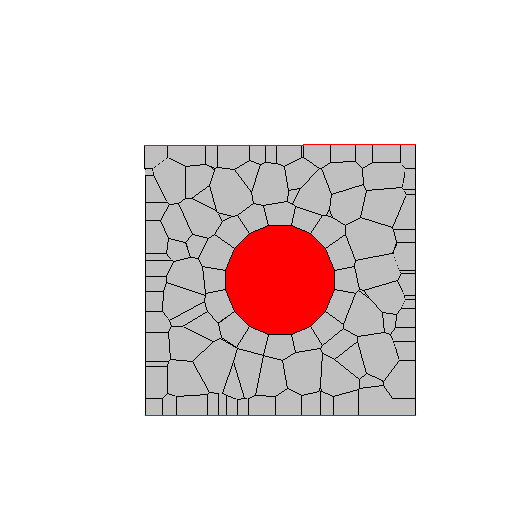
\includegraphics[width=0.4\linewidth]{Files/Small_ASR/CR/DEP5-STEP(001).png}
%*******
\caption{Single Aggregate Case in Size $10 \times 10 \times 10$ mm}
\label{mmmm}
\end{figure}


The expanse is generated at the location of interfaces between mortar and mortar elements, to introduce the expansion, as mentioned in chapter 2.

As the model is small in size, and it is a representation of the expansion in part of the whole structure in theoretically, uniform expansion is applied here.

%TODO: Single Aggregate 3D, 2D

0.0003 initial strain is introduced in each step at the interfaces between the paste and paste elements. Totally 20 steps of expansion are done.

% Small DEF CR
  \begin{figure}[ht!]
  \centering
      %*******
      \begin{subfigure}{.25\textwidth}
        \centering
        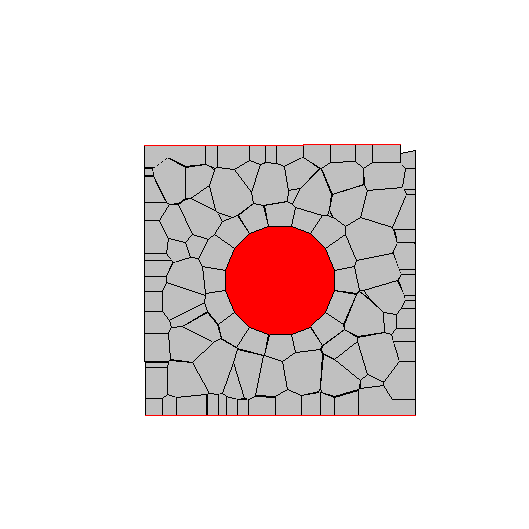
\includegraphics[width=1.0\linewidth]{Files/Small_DEF/CR/DEP5-STEP(001).png}
      \caption{Step 1}
      \end{subfigure}%
      %*******
      \begin{subfigure}{.25\textwidth}
        \centering
        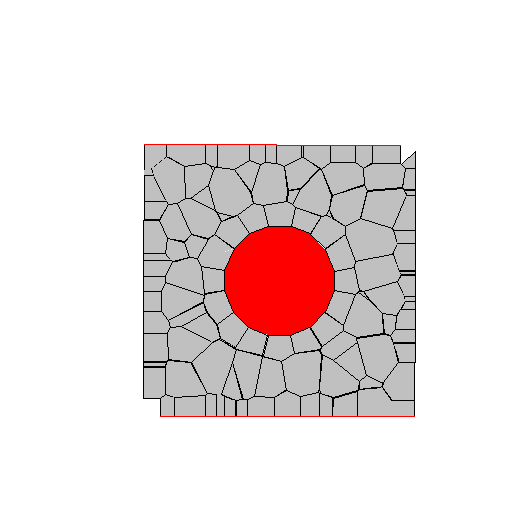
\includegraphics[width=1.0\linewidth]{Files/Small_DEF/CR/DEP5-STEP(002).png}
      \caption{Step 2}
      \end{subfigure}%
      %*******
      \begin{subfigure}{.25\textwidth}
        \centering
        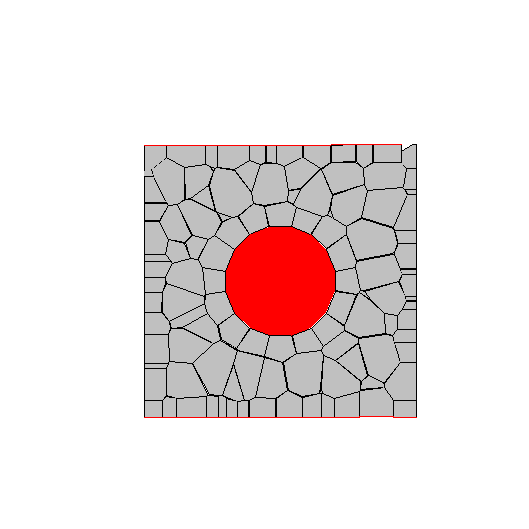
\includegraphics[width=1.0\linewidth]{Files/Small_DEF/CR/DEP5-STEP(003).png}
      \caption{Step 3}
      \end{subfigure}%
      %*******
      \begin{subfigure}{.25\textwidth}
        \centering
        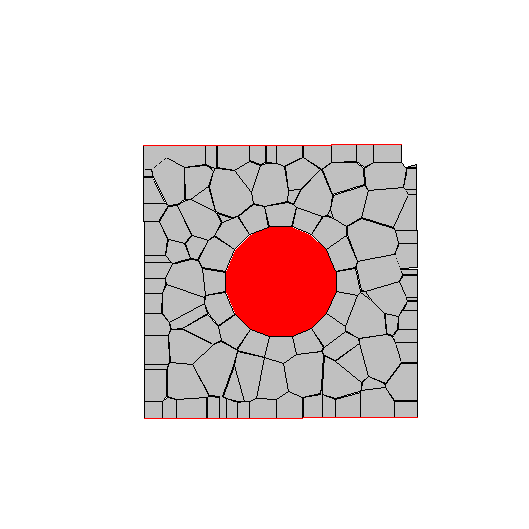
\includegraphics[width=1.0\linewidth]{Files/Small_DEF/CR/DEP5-STEP(004).png}
      \caption{Step 4}
      \end{subfigure}

      %*******
      %*******
      \begin{subfigure}{.25\textwidth}
        \centering
        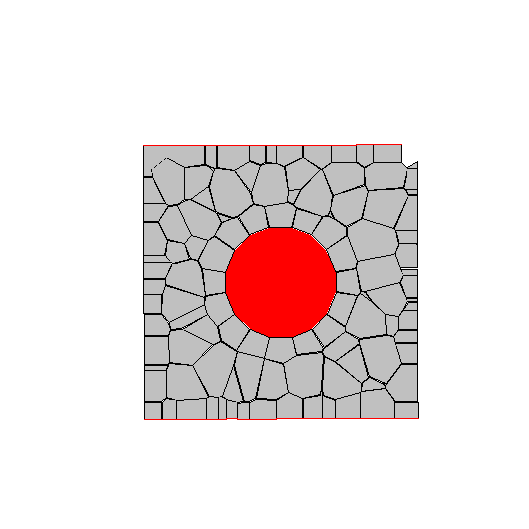
\includegraphics[width=1.0\linewidth]{Files/Small_DEF/CR/DEP5-STEP(005).png}
      \caption{Step 5}
      \end{subfigure}%
      %*******
      \begin{subfigure}{.25\textwidth}
        \centering
        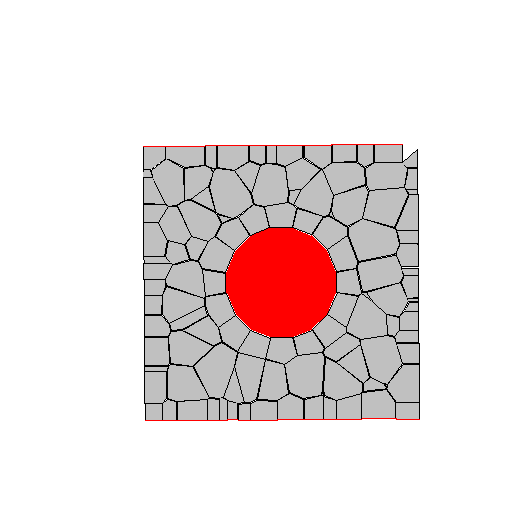
\includegraphics[width=1.0\linewidth]{Files/Small_DEF/CR/DEP5-STEP(006).png}
      \caption{Step 6}
      \end{subfigure}%
      %*******
      \begin{subfigure}{.25\textwidth}
        \centering
        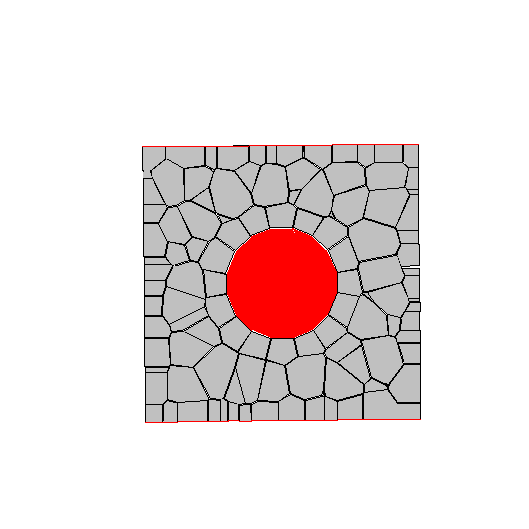
\includegraphics[width=1.0\linewidth]{Files/Small_DEF/CR/DEP5-STEP(007).png}
      \caption{Step 7}
      \end{subfigure}%
      %*******
      \begin{subfigure}{.25\textwidth}
        \centering
        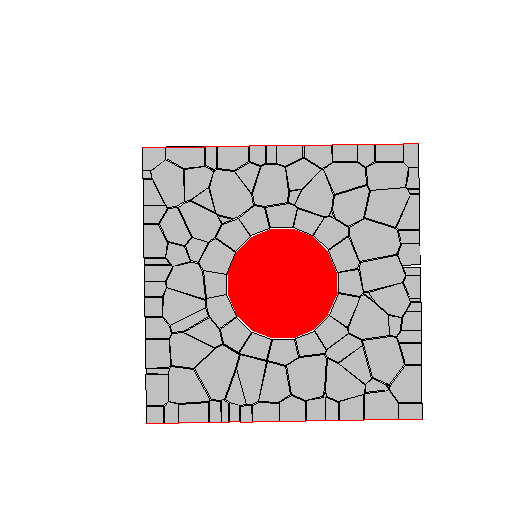
\includegraphics[width=1.0\linewidth]{Files/Small_DEF/CR/DEP5-STEP(008).png}
      \caption{Step 4}
      \end{subfigure}

      %*******
      %*******
      \begin{subfigure}{.25\textwidth}
        \centering
        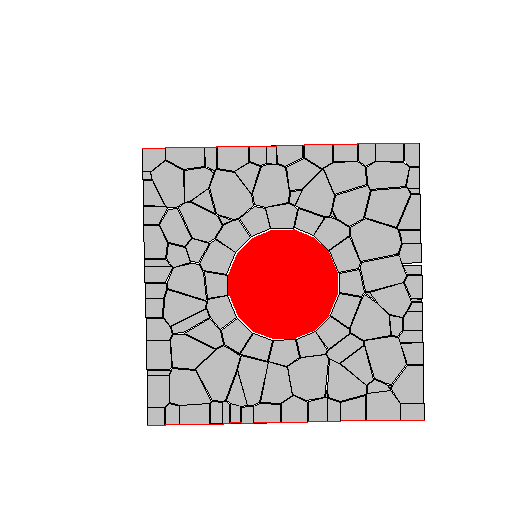
\includegraphics[width=1.0\linewidth]{Files/Small_DEF/CR/DEP5-STEP(009).png}
      \caption{Step 9}
      \end{subfigure}%
      %*******
      \begin{subfigure}{.25\textwidth}
        \centering
        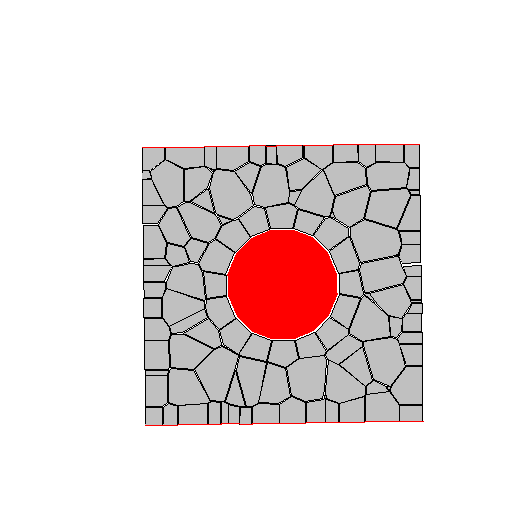
\includegraphics[width=1.0\linewidth]{Files/Small_DEF/CR/DEP5-STEP(010).png}
      \caption{Step 10}
      \end{subfigure}%
      %*******
      \begin{subfigure}{.25\textwidth}
        \centering
        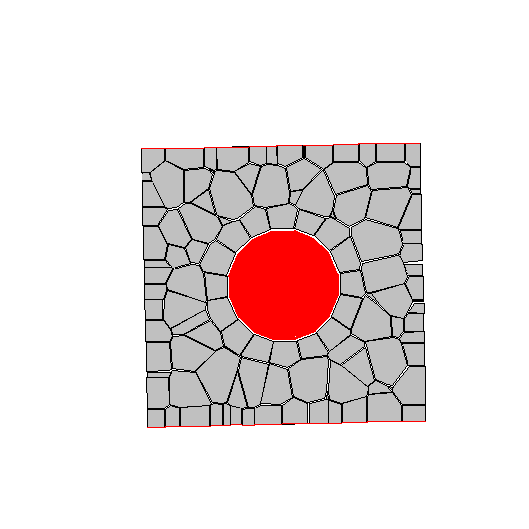
\includegraphics[width=1.0\linewidth]{Files/Small_DEF/CR/DEP5-STEP(011).png}
      \caption{Step 11}
      \end{subfigure}%
      %*******
      \begin{subfigure}{.25\textwidth}
        \centering
        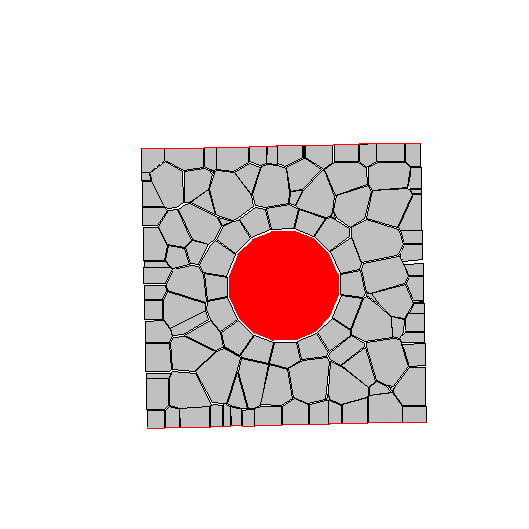
\includegraphics[width=1.0\linewidth]{Files/Small_DEF/CR/DEP5-STEP(012).png}
      \caption{Step 12}
      \end{subfigure}

      %*******
      %*******
      \begin{subfigure}{.25\textwidth}
        \centering
        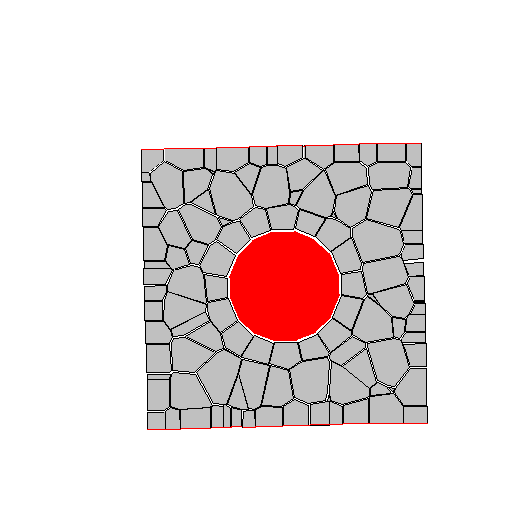
\includegraphics[width=1.0\linewidth]{Files/Small_DEF/CR/DEP5-STEP(013).png}
      \caption{Step 13}
      \end{subfigure}%
      %*******
      \begin{subfigure}{.25\textwidth}
        \centering
        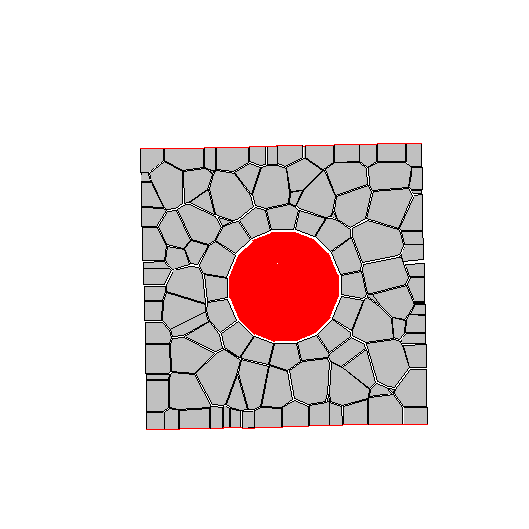
\includegraphics[width=1.0\linewidth]{Files/Small_DEF/CR/DEP5-STEP(014).png}
      \caption{Step 14}
      \end{subfigure}%
      %*******
      \begin{subfigure}{.25\textwidth}
        \centering
        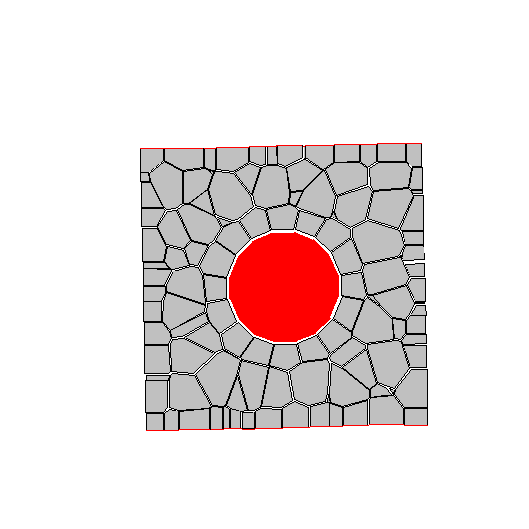
\includegraphics[width=1.0\linewidth]{Files/Small_DEF/CR/DEP5-STEP(015).png}
      \caption{Step 15}
      \end{subfigure}%
      %*******
      \begin{subfigure}{.25\textwidth}
        \centering
        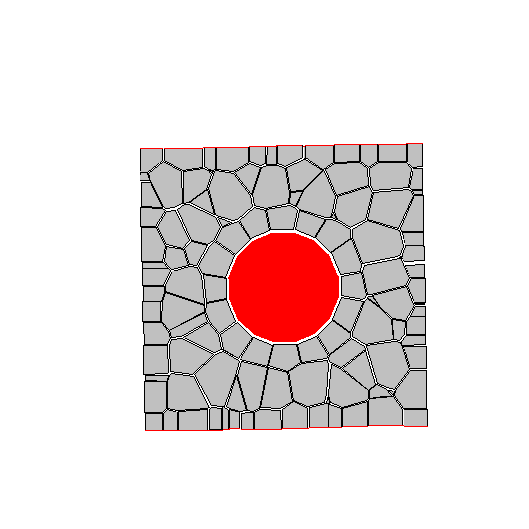
\includegraphics[width=1.0\linewidth]{Files/Small_DEF/CR/DEP5-STEP(016).png}
      \caption{Step 16}
      \end{subfigure}

      %*******
      %*******
      \begin{subfigure}{.25\textwidth}
        \centering
        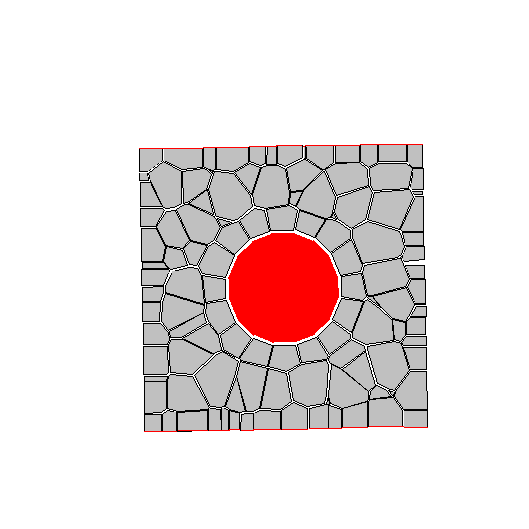
\includegraphics[width=1.0\linewidth]{Files/Small_DEF/CR/DEP5-STEP(017).png}
      \caption{Step 17}
      \end{subfigure}%
      %*******
      \begin{subfigure}{.25\textwidth}
        \centering
        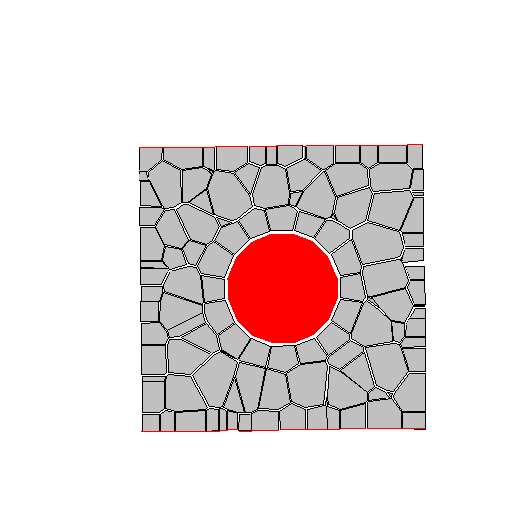
\includegraphics[width=1.0\linewidth]{Files/Small_DEF/CR/DEP5-STEP(018).png}
      \caption{Step 18}
      \end{subfigure}%
      %*******
      \begin{subfigure}{.25\textwidth}
        \centering
        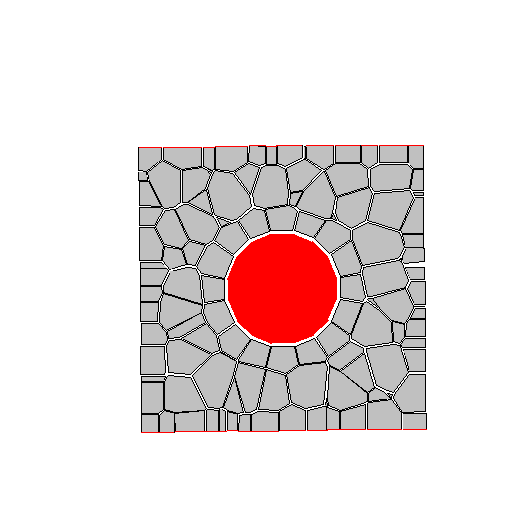
\includegraphics[width=1.0\linewidth]{Files/Small_DEF/CR/DEP5-STEP(019).png}
      \caption{Step 19}
      \end{subfigure}%
      %*******
      \begin{subfigure}{.25\textwidth}
        \centering
        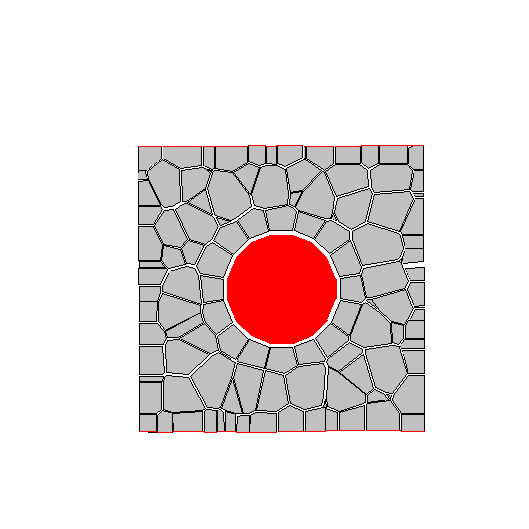
\includegraphics[width=1.0\linewidth]{Files/Small_DEF/CR/DEP5-STEP(020).png}
      \caption{Step 20}
      \end{subfigure}

  \caption{Internal Stress in Each Step for DEF $10 \times 10 \times 10$ mm Case ($Deformation \times 10$)}
  \label{fig:DEF_Small_DEF_CR}
  \end{figure}

From the Figure \ref{fig:DEF_Small_DEF_CR}, we can see that step by step with initial stain introducing into the model, distance appears between aggregate and the surrounding element at first, meanwhile the distance between paste elements open gradually as we increase the step of expansion.

As the paste apart from aggregate in the center, there is no compressive or tension stress appearing in the aggregate.

Not like the case of ASR, the DEF expansion here have relatively uniformed opening in all paste parts.

The total volume of this small model is increasing step by step, while until the step 20 the model expanded 0.6098\% one-dimensionally.

% Small DEF IS
  \begin{figure}[ht!]
  \centering
      %*******
      \begin{subfigure}{.25\textwidth}
        \centering
        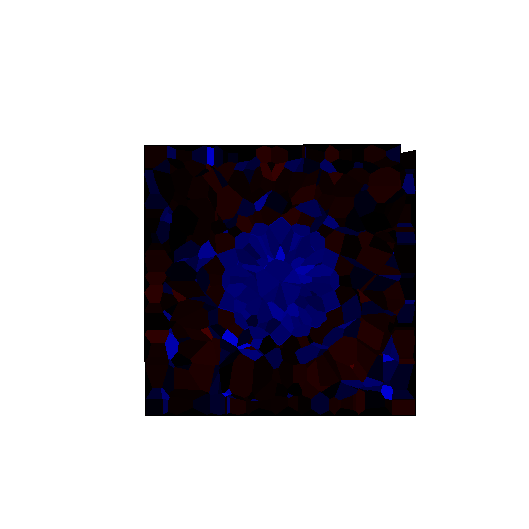
\includegraphics[width=1.0\linewidth]{Files/Small_DEF/IS/DEP5-STEP(001).png}
      \caption{Step 1}
      \end{subfigure}%
      %*******
      \begin{subfigure}{.25\textwidth}
        \centering
        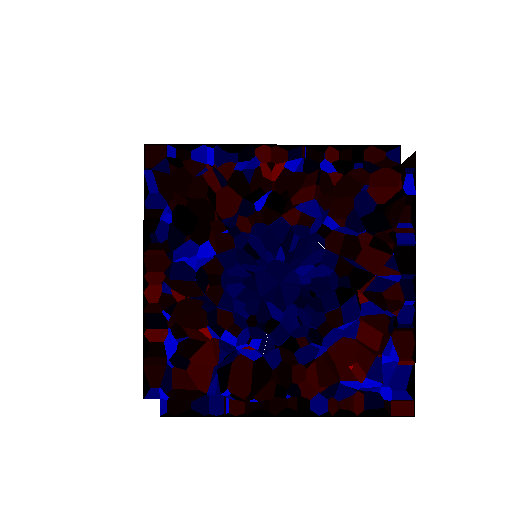
\includegraphics[width=1.0\linewidth]{Files/Small_DEF/IS/DEP5-STEP(002).png}
      \caption{Step 2}
      \end{subfigure}%
      %*******
      \begin{subfigure}{.25\textwidth}
        \centering
        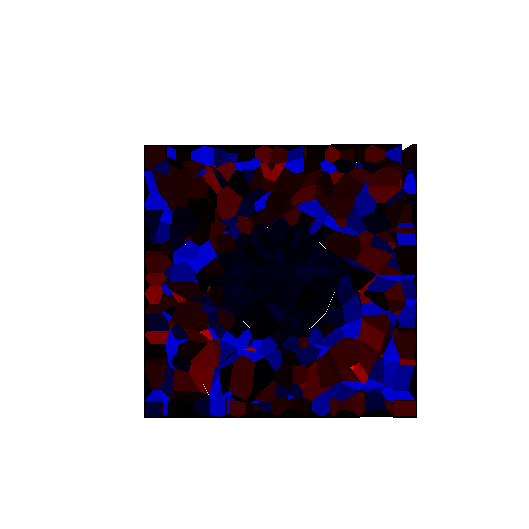
\includegraphics[width=1.0\linewidth]{Files/Small_DEF/IS/DEP5-STEP(003).png}
      \caption{Step 3}
      \end{subfigure}%
      %*******
      \begin{subfigure}{.25\textwidth}
        \centering
        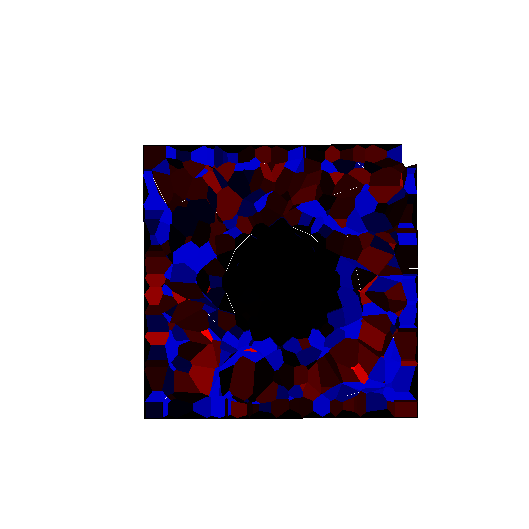
\includegraphics[width=1.0\linewidth]{Files/Small_DEF/IS/DEP5-STEP(004).png}
      \caption{Step 4}
      \end{subfigure}

      %*******
      %*******
      \begin{subfigure}{.25\textwidth}
        \centering
        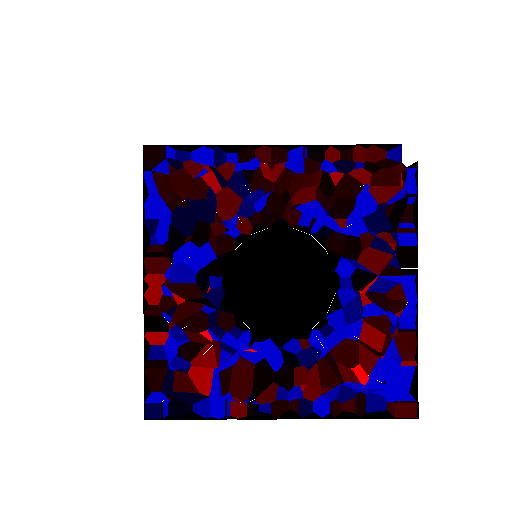
\includegraphics[width=1.0\linewidth]{Files/Small_DEF/IS/DEP5-STEP(005).png}
      \caption{Step 5}
      \end{subfigure}%
      %*******
      \begin{subfigure}{.25\textwidth}
        \centering
        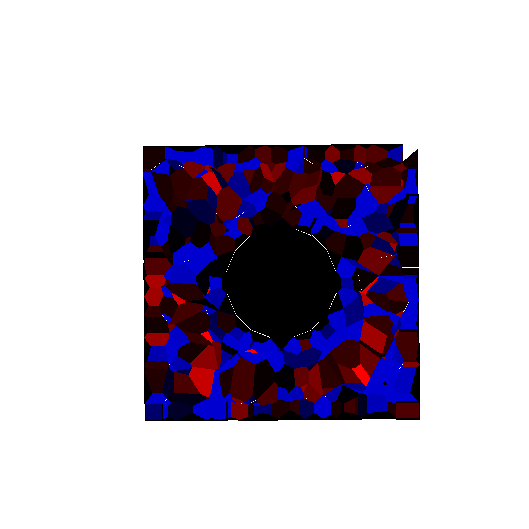
\includegraphics[width=1.0\linewidth]{Files/Small_DEF/IS/DEP5-STEP(006).png}
      \caption{Step 6}
      \end{subfigure}%
      %*******
      \begin{subfigure}{.25\textwidth}
        \centering
        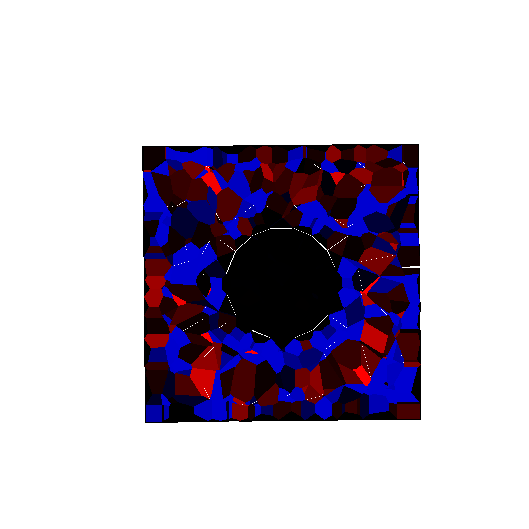
\includegraphics[width=1.0\linewidth]{Files/Small_DEF/IS/DEP5-STEP(007).png}
      \caption{Step 7}
      \end{subfigure}%
      %*******
      \begin{subfigure}{.25\textwidth}
        \centering
        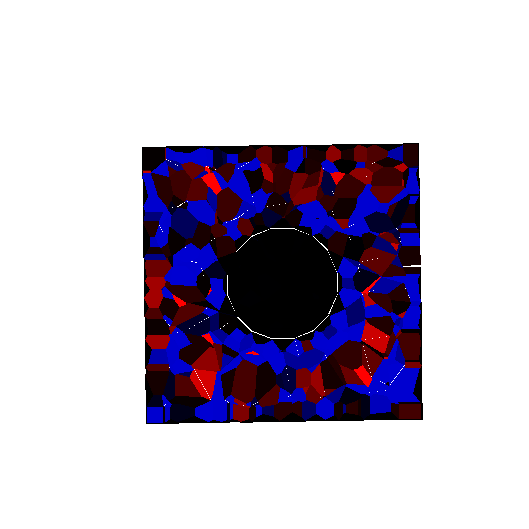
\includegraphics[width=1.0\linewidth]{Files/Small_DEF/IS/DEP5-STEP(008).png}
      \caption{Step 4}
      \end{subfigure}

      %*******
      %*******
      \begin{subfigure}{.25\textwidth}
        \centering
        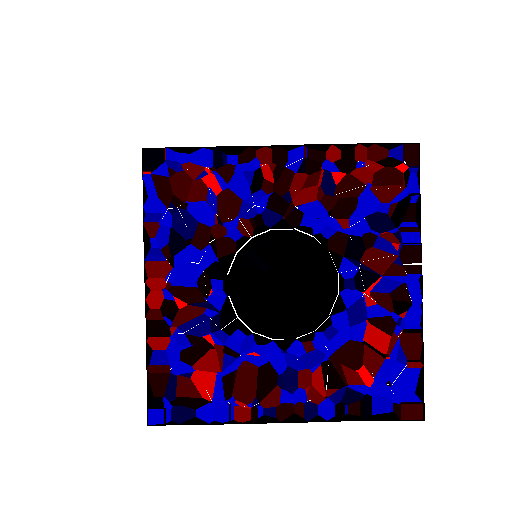
\includegraphics[width=1.0\linewidth]{Files/Small_DEF/IS/DEP5-STEP(009).png}
      \caption{Step 9}
      \end{subfigure}%
      %*******
      \begin{subfigure}{.25\textwidth}
        \centering
        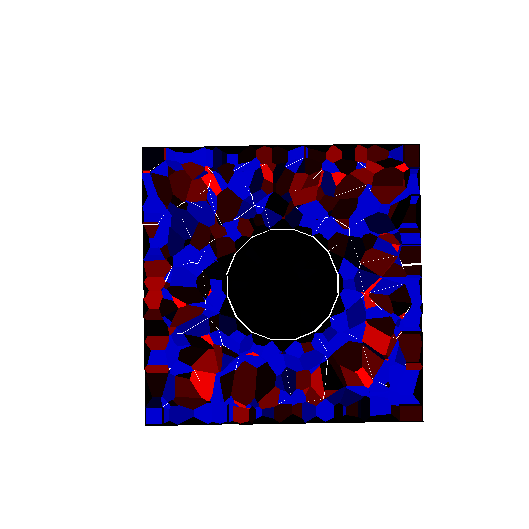
\includegraphics[width=1.0\linewidth]{Files/Small_DEF/IS/DEP5-STEP(010).png}
      \caption{Step 10}
      \end{subfigure}%
      %*******
      \begin{subfigure}{.25\textwidth}
        \centering
        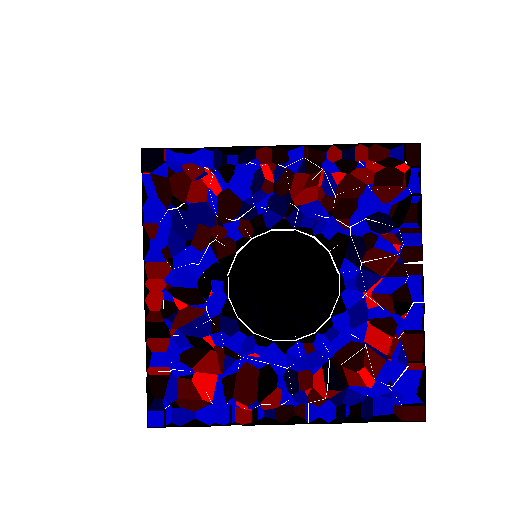
\includegraphics[width=1.0\linewidth]{Files/Small_DEF/IS/DEP5-STEP(011).png}
      \caption{Step 11}
      \end{subfigure}%
      %*******
      \begin{subfigure}{.25\textwidth}
        \centering
        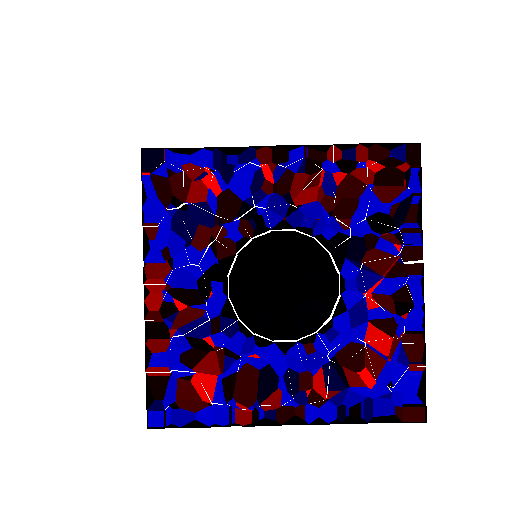
\includegraphics[width=1.0\linewidth]{Files/Small_DEF/IS/DEP5-STEP(012).png}
      \caption{Step 12}
      \end{subfigure}

      %*******
      %*******
      \begin{subfigure}{.25\textwidth}
        \centering
        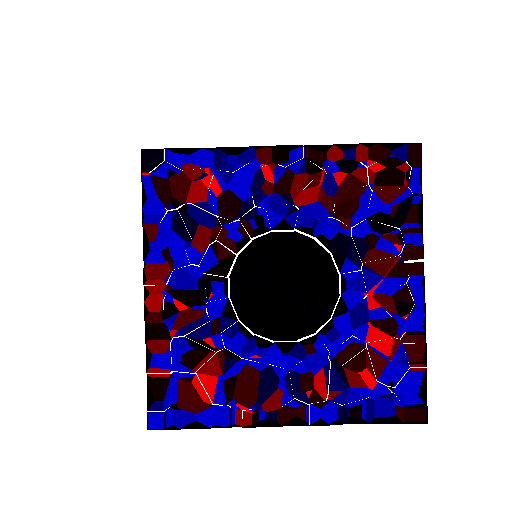
\includegraphics[width=1.0\linewidth]{Files/Small_DEF/IS/DEP5-STEP(013).png}
      \caption{Step 13}
      \end{subfigure}%
      %*******
      \begin{subfigure}{.25\textwidth}
        \centering
        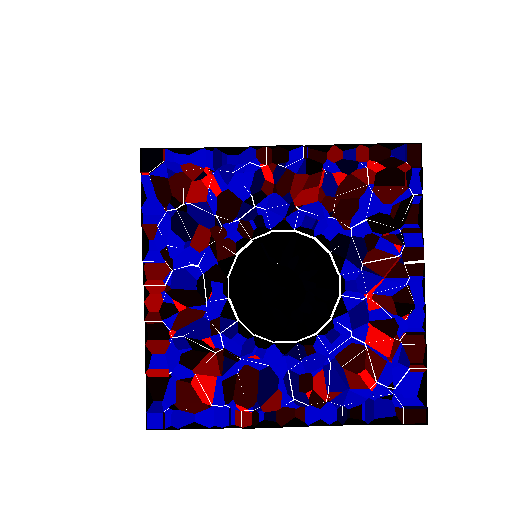
\includegraphics[width=1.0\linewidth]{Files/Small_DEF/IS/DEP5-STEP(014).png}
      \caption{Step 14}
      \end{subfigure}%
      %*******
      \begin{subfigure}{.25\textwidth}
        \centering
        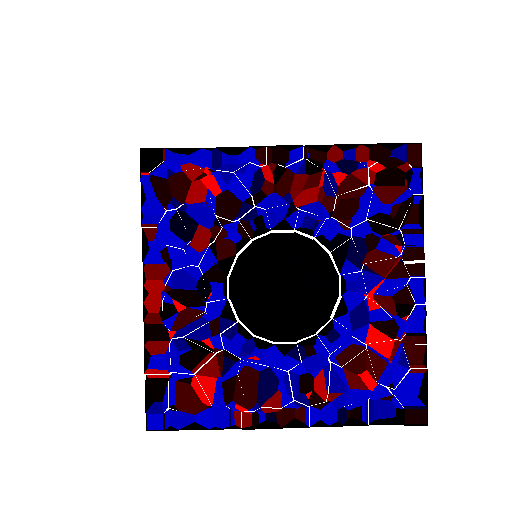
\includegraphics[width=1.0\linewidth]{Files/Small_DEF/IS/DEP5-STEP(015).png}
      \caption{Step 15}
      \end{subfigure}%
      %*******
      \begin{subfigure}{.25\textwidth}
        \centering
        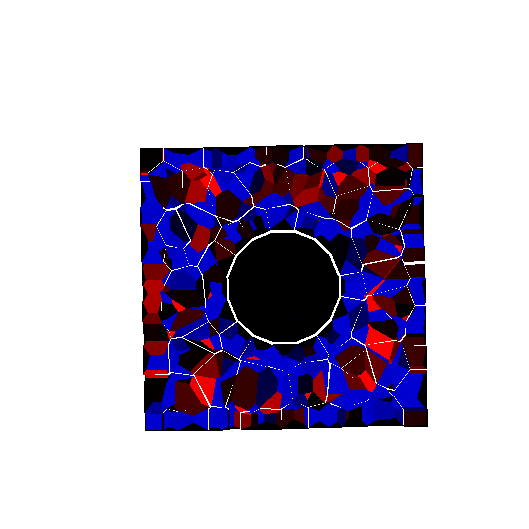
\includegraphics[width=1.0\linewidth]{Files/Small_DEF/IS/DEP5-STEP(016).png}
      \caption{Step 16}
      \end{subfigure}

      %*******
      %*******
      \begin{subfigure}{.25\textwidth}
        \centering
        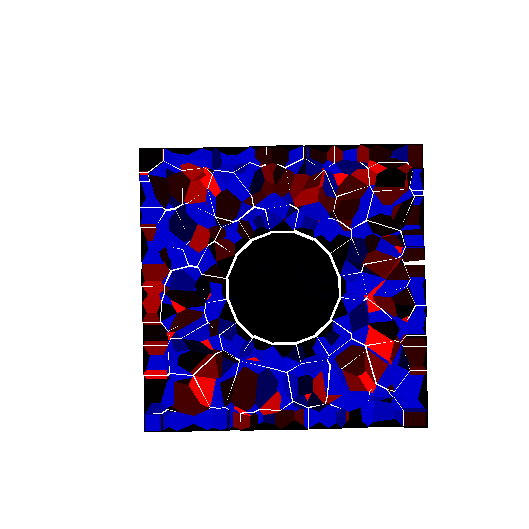
\includegraphics[width=1.0\linewidth]{Files/Small_DEF/IS/DEP5-STEP(017).png}
      \caption{Step 17}
      \end{subfigure}%
      %*******
      \begin{subfigure}{.25\textwidth}
        \centering
        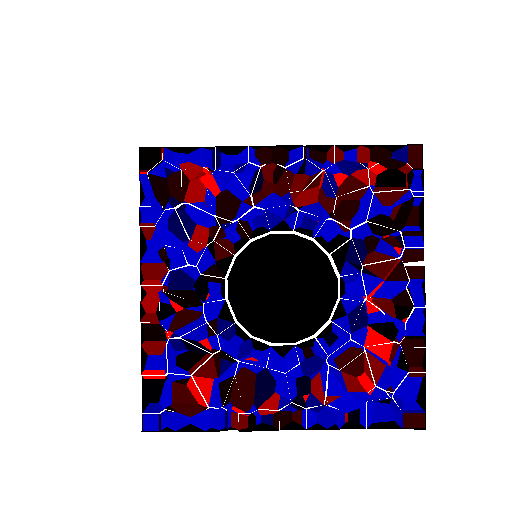
\includegraphics[width=1.0\linewidth]{Files/Small_DEF/IS/DEP5-STEP(018).png}
      \caption{Step 18}
      \end{subfigure}%
      %*******
      \begin{subfigure}{.25\textwidth}
        \centering
        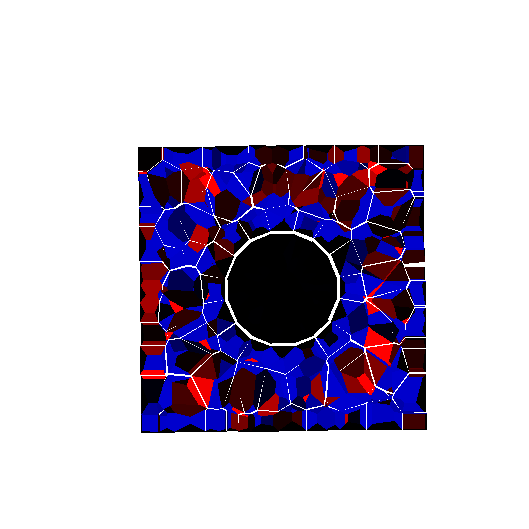
\includegraphics[width=1.0\linewidth]{Files/Small_DEF/IS/DEP5-STEP(019).png}
      \caption{Step 19}
      \end{subfigure}%
      %*******
      \begin{subfigure}{.25\textwidth}
        \centering
        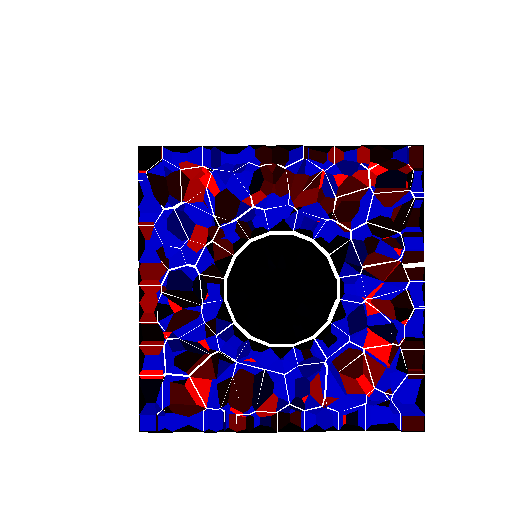
\includegraphics[width=1.0\linewidth]{Files/Small_DEF/IS/DEP5-STEP(020).png}
      \caption{Step 20}
      \end{subfigure}

      \begin{subfigure}{0.8\textwidth}
  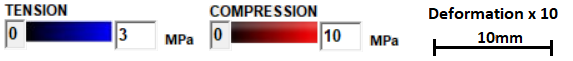
\includegraphics[width=0.8\linewidth]{Files/exp_3D/tagCS10s.png}
\end{subfigure}%


  \caption{Internal Stress in Each Step for DEF $10 \times 10 \times 10$ mm Case ($Deformation \times 10$)}
  \label{fig:DEF_Small_DEF_IS}
  \end{figure}

Also, the Inner Stress condition for each step is collected, and shown in Figure \ref{fig:DEF_Small_DEF_IS}.

As shown in the inner stress condition, at the beginning of the expansion, the aggregate is under tensile stress and paste parts surrounding is under compression. Since the initial strain is given to the paste, with the increasing of initial strain by each step, the compressive stress accumulates in the paste part. While for the aggregate, after gap developed between aggregate and paste around it, the aggregate is not suffering from tension or compression.

This very small size simple example shows that, same as ASR case, logically our method of adding initial strain to generate DEF expansion should work in the way we assumed.
